\chapter{Architecture / Implementation}
\label{ch:implementation}

\begin{figure}[ht]
	% \centering
	\hspace*{-0.5cm}
	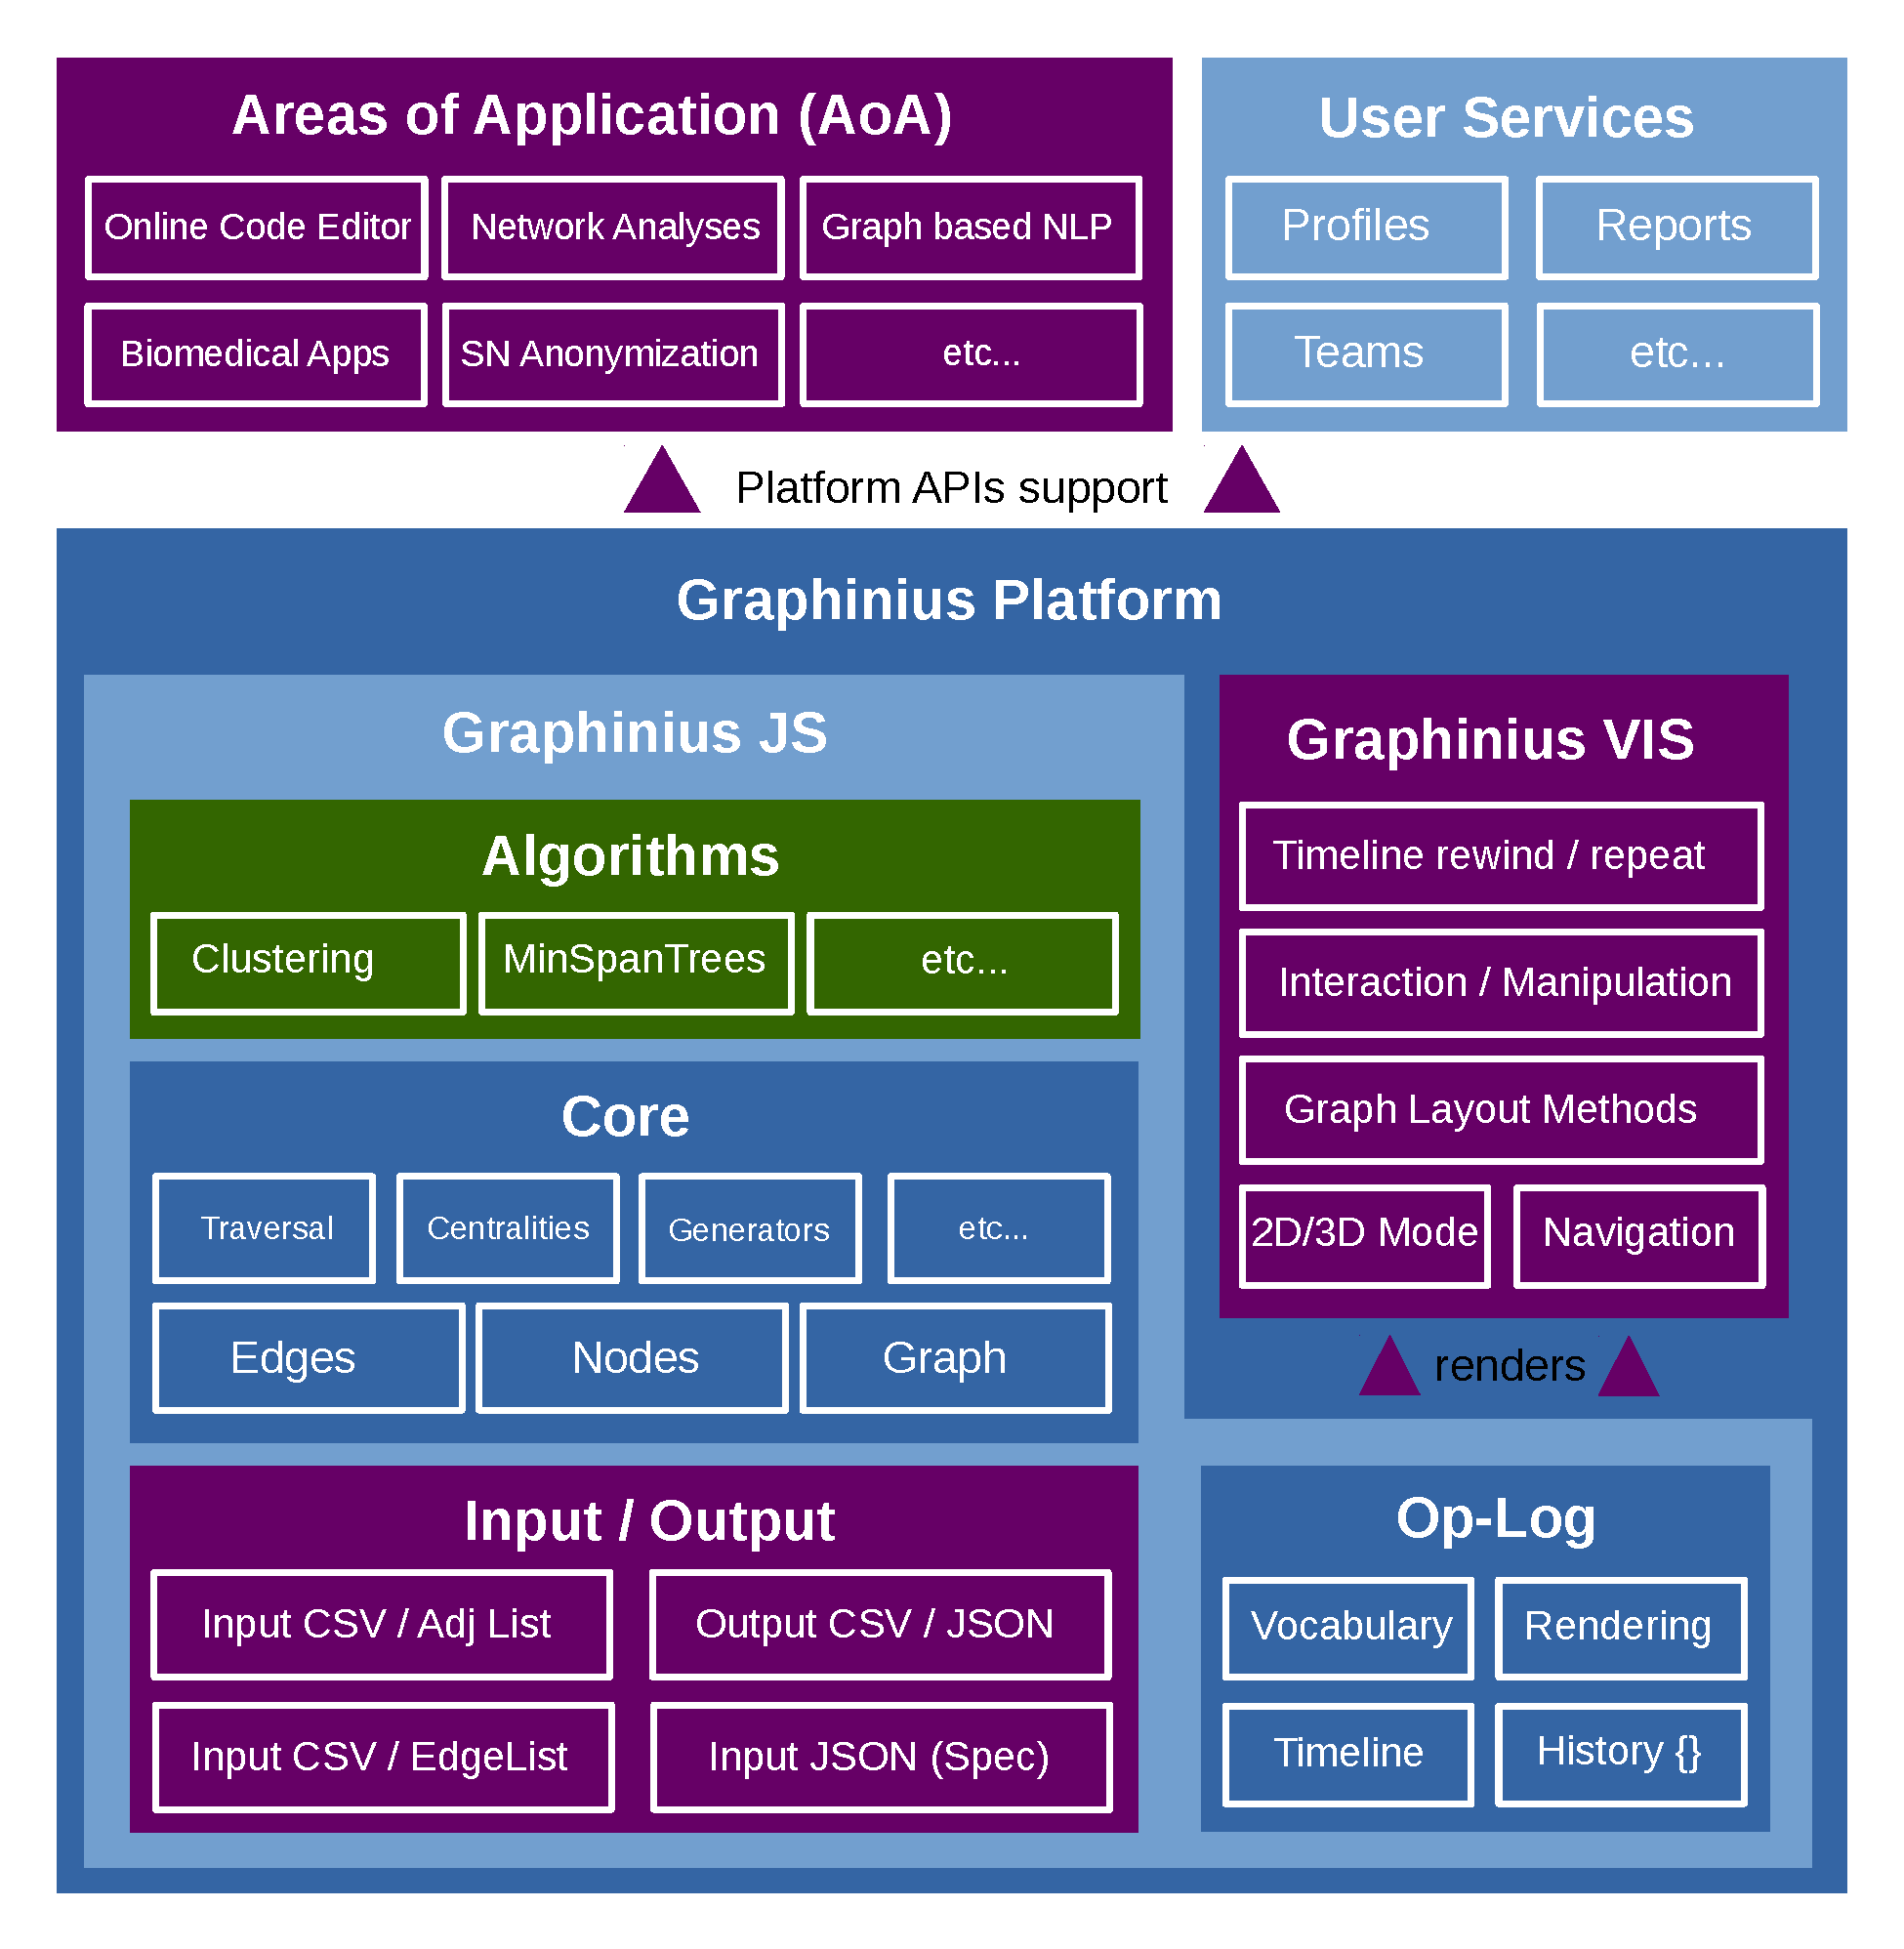
\includegraphics[width=1.1\textwidth]{figures/Graphinius_Architecture_pdf}
	\caption{Graphinius platform architecture overview}
	\label{fig_graphinius_architecture}
\end{figure}


\section{Graphinius Base}
\label{sect:graphinius_base}

As the name suggests, the Base offers all the functionality necessary to develop graph-based applications on top of it, including basic graph-computations and algorithms as well as visualization. It is therefore logically composed of those two modules, Graphinius JS and Graphinius VIS as well as a mechanism of communication between those two.


\section{Graphinius JS}
\label{sect:graphinius_js}

	\subsection{Graph Core}
	\label{ssect:graph_core}
		
		\subsubsection{Edges}
		\label{sssection: core_edges}
		
		\subsubsection{Nodes}
		\label{sssection: core_nodes}
		
		\subsubsection{Graph}
		\label{sssection: core_graph}
		
		\subsubsection{Traversal}
		\label{sssection: core_traveral}
		
		BFS / DFS implementations... [figure: callback-based DFS]
		
		\subsubsection{Degrees}
		\label{sssection: core_degrees}
		
		\subsubsection{Generators}
		\label{sssection: core_}
		
		probability
		per-node degree

	
	\subsection{Graph input readers}
	\label{ssect:input_output}
		
		\subsubsection{CSV}
		\label{sssection: io_csv}
		
		
		\begin{figure}[ht]
			\begin{lstlisting}
			A, B, u, C, u, A, d, B, d, D, d
			B, A, u
			C, A, u, A, d
			D, A, d
			\end{lstlisting}
			\caption{Adjacency list including edge direction}
			\label{fig:adj_list_direction}
		\end{figure}
		
		CSV Edge Lists use the simple format of [StartNode, EndNode [,directed]].		
		
		
		\subsubsection{JSON}
		\label{sssection: io_json}
		
		\begin{figure}[ht]
			\centering
			\hspace*{-1.5cm}
			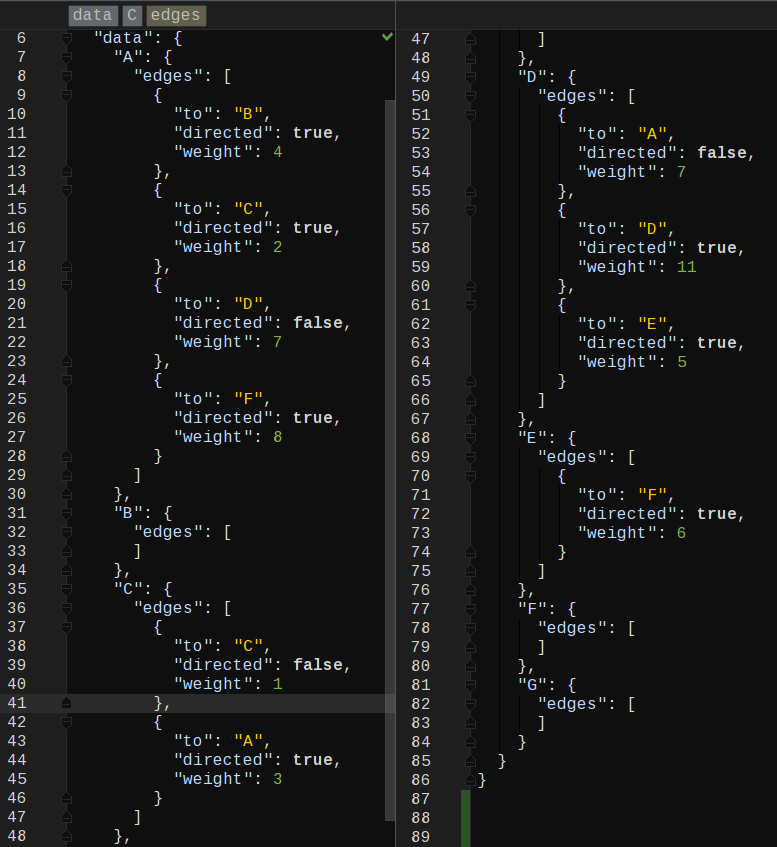
\includegraphics[width=1.2\textwidth]{figures/search_graph_json}
			\caption{Sample graph in the Graphinius JSON format}
			\label{fig:json_input_graph}
			\small Apart from the 'to' node, direction and weight, any node can exhibit an arbitrarily large feature vector containing any type of information (like patient data, word vectors, etc.). Another special sub-object which the input reader is looking for is the 'coords' object, which specifies the coordinates used in the constant layout renderer of the GraphiniusVIS library.
		\end{figure}



\section{The Op-Log / History system}
\label{sect:op_log}

	The idea of a history subsystem came from the concept of a real-time in-browser graph exploration platform, in which every action performed via an online editor or some GUI action should result in some immediate, visible change in the graph visualization. Ideally, such real-time changes would also be reversible, so that a user could progress step-by-step forward and backward in time - either to grasp more clearly what some algorithm does to the structure of a graph, or to 'simulate' the behavior of an algorithm on the whole. 
	
	In order to guarantee smooth behavior as well as separation of concerns in the software, placing this functionality directly in either the GraphiniusJS or GraphiniusVIS libraries would violate sound architectural principles. Therefor, the author proposes (but has not implemented yet) the following general module:
	
	\begin{landscape}
		\begin{figure}[ht]
			\label{fig_history_workflow}
			\centering
			\vspace{-2.0cm}
			%	\hspace*{0cm}
			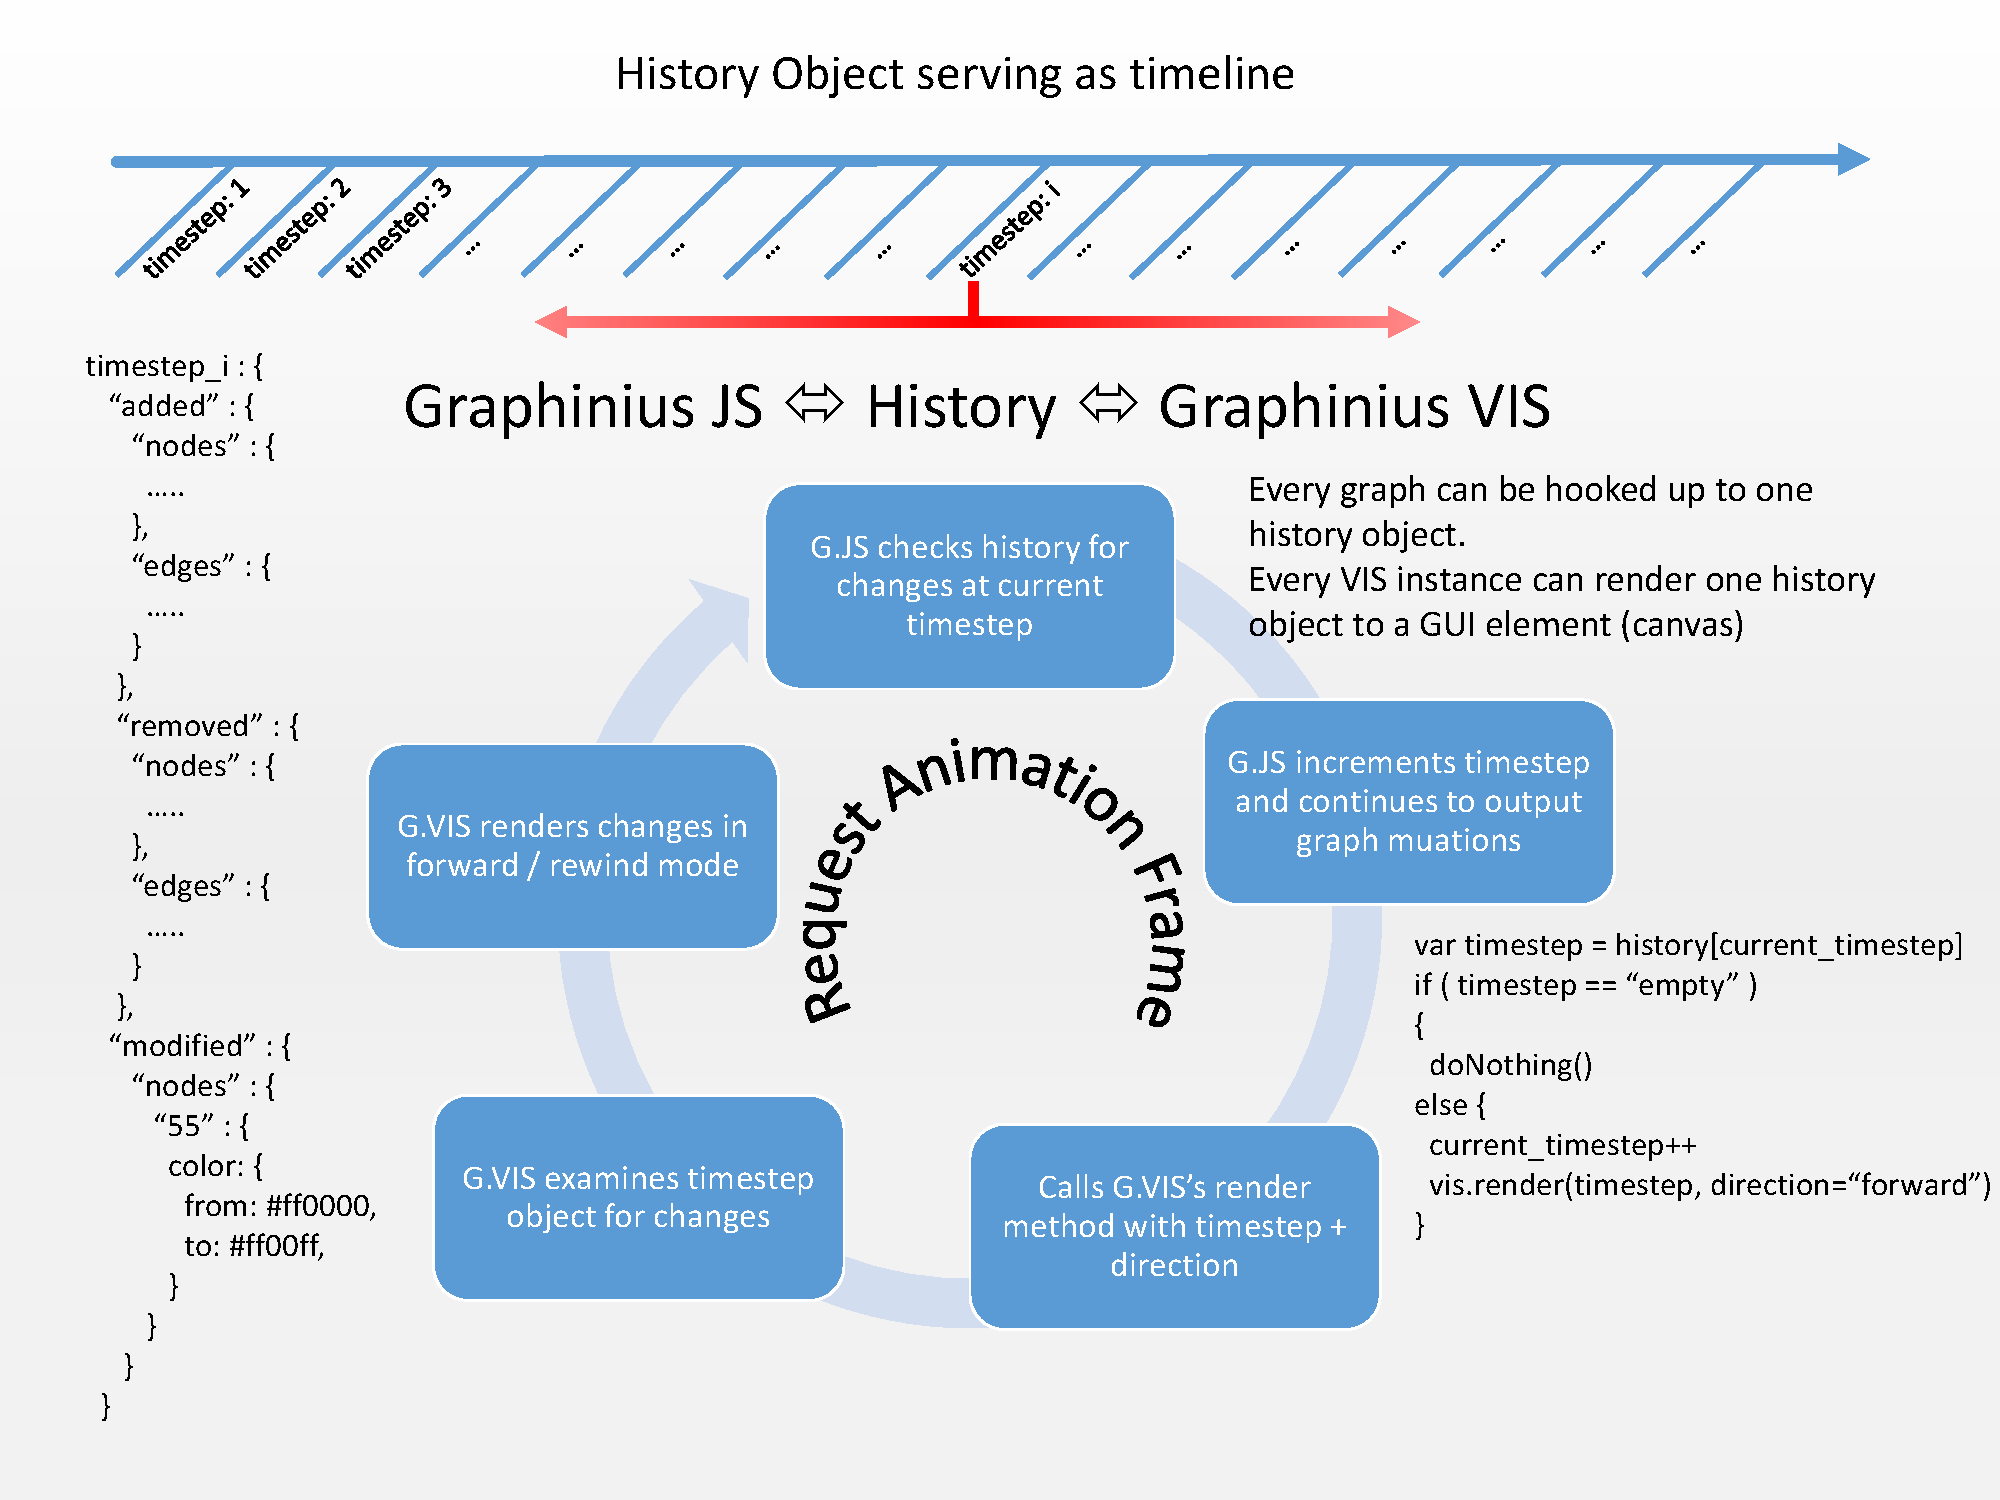
\includegraphics[width=1.6\textwidth]{figures/History_Workflow_pdf}
			\caption{Graphinius JS <-> VIS communication via Op-Log}
		\end{figure}
	\end{landscape}

	\subsection{Timeline}
	\label{ssect:timeline}
	
	The basic idea in implementing the system is to organize all graph mutations along the time axis, if only to imply chronological order. While it is less important to be able to specifically 'audit' some action in the sense of being able to exactly locate its temporal occurrence, we need some mapping of actions to a timestep (object) in order to be able to traverse the timeline back and forth. This is what determines the structure of the history object.
	
	\subsection{History Object}
	\label{ssect:history_object}

	The history object is a simple JavaScript object (which behaves like a hashmap in other languages' vocabulary) and holds entries in the form of \textit{timestep(timestep:number => actions:JSObject)}. These actions sub-objects then contain all the mutations which took place at a certain \textit{timestep}. It is important to realize that this \textit{timestep} is not an exact moment in time, but can span an arbitrarily long interval. Its value is determined by a global \textit{timestep} variable, which is only incremented when the rendering of the currently 'active' timestep has commenced. The actual procedure take the form of the following loop:
	
	\begin{enumerate}
		\item Graphinius Platforms runs recursive calls to \textit{window.requestAnimationFrame(renderFunc)} which simulates a main GUI loop
		\item At the beginning of each invocation, the algorithm checks for the current value of the global \textit{timestep} variable, and checks if the respective entry in the history object is empty or populated.
		\item In case it is empty, the algorithm breaks, laying inactive until the next time-tick from requestAnimationFrame (16.67 milliseconds on a 60Hz monitor).
		\item In case it is populated, the algorithm increments the global \textit{timestep} value - from this point onwards, GraphiniusJS will not write to that entry any more ('locking' it so that the rendering process can finish).
		\item All items in the current \textit{timestep} object will be evaluated resulting in calls to the GraphiniusVIS library updating the in-browser visualization.
	\end{enumerate}
	
	In order to be able to replay / rewind the mechanism, the history subsystem must have a sense of direction in time - which in our case simply translates to possessing a vocabulary expressing graph mutations in such a way that the respective inverse function is easily obtainable.
	
	\subsection{Vocabulary}
	\label{ssect:vocabulary}
	
	In order to achieve this, the \textit{timestep} entries must be as simple and specific as possible. For most of the primitive graph mutations, this is practically going to happen automatically: For instance, given the command \textit{'addNode(nodeId, arguments)'}, the inverse is logically \textit{'deleteNode(nodeId)'}. For more complex actions like changing coordinates, colors or shape, the original values would have to be stored. In the case of actions regarding whole clusters or changing the structure of the entire graph (\textit{run mincut..}), the \textit{timestep} entries will have to be broken down into atomic units and inverse actions defined in beforehand.


\section{Graphinius VIS}
\label{sect:graphinius_vis}

	The author was fortunate to receive the opportunity to guide the Master's Project of Nicole Neuhold in implementing a visualization module for the emerging Graphinius platform. We were working on research, experiments, and the foundation of a future implementation from early January 2016 to the end of March of the same year, and I am proud to be able to say that we surpassed our initial expectations - in brevity and conciseness of implementation as well as performance - by leaps and bounds and are not able to visualize graphs of 15k nodes / 40k edges fluently (~25 FPS) even on middle class laptops (22k nodes / 65k edges fluently on the author's desktop machine featuring a low-middle-class Geforce 650TI with 2GB of video RAM).
	
	\subsection{WebGL rendering}
	\label{ssect:webgl_rendering}
	
	The core component of the GraphiniusVIS module is the WebGL renderer. Although we experimented with SVG and Canvas (2D) as well, we quickly realized that both alternatives were either too slow or didn't provide us with the experience we desired: SVG has the great advantage of working with normal browser (DOM) objects, which enables easy interaction and selection via JS / CSS selectors, but stops rendering fluently at only a few hundred nodes / a few thousand edges.
	
	Canvas, on the other hand, is fine and fast enough for visualizing logical graph structures of thousands of nodes / edges in 2D. Nevertheless, because our project originated from the need to render structures  inherently 3D (like nevi and organs) and there was no easy possibility to project a 3D space onto a 2D canvas (except for computing the projection ourselves), we finally decided against it.
	
	Our Three.js / WebGL based renderer now uses low-level data structures like buffer geometries, statically typed JavaScript arrays and particle systems instead of 3D objects for nodes, which enables us to transfer our (pre-)computed data to the GPU in one single copy operation - this alone increases performance easily 10-fold over earlier attempts at progressively adding new objects to the scene.
	
	\subsection{2D/3D Mode}
	\label{ssect:vis_2d3d}
	
	GraphiniusVIS supports both 2D and 3D visualization of graph structures. However, since we are using WebGL which is inherently 3D, when switching to 2D mode we are not falling back to SVG or canvas but instead just 'fix' all z-coordinates of nodes / edges to zero, so we end up with a 2D object floating in 3D space.
	
	\subsection{Navigation}
	\label{ssect:vis_navigation}
	
	Our module supports panning (via mouse click-and-move), zooming (via mouse-wheel), rotating (via Shift + mouse click-and-move), and also provides any of those actions via keyboard commands.
	
	\subsection{Graph Layouts}
	\label{ssect:vis_layouts}
	
	The field of graph drawing has been an active area of research for several decades now, and many graph layouts have been developed for diverse areas of applications. Apart from constant (coordinate-based) layouts and force-directed layouts for physical simulations, there exist circular, spherical, tree-based, and arc diagrams, to name only a tiny fraction. Our basic implementation supports a constant layout per default, and allows switching to a force-directed layout as well, although the latter is currently implemented as a simple mathematical sine function instead of making use of attracting / repulsive forces.
	
	\subsection{Interaction / Manipulation}
	\label{ssect:vis_interact_manipulate}
	
	There are almost endless possibilities to interact with and manipulate a graph structure, so we were limited to offering just a small selection in order to demonstrate the viability of our GraphiniusVIS module. We chose to implement node and edge addition as well as deletion, changing the color of nodes and edges, updating their coordinates as well as switching from constant to our (simplified) force-directed layout. 
	
	In addition to that, in order to demonstrate seemless interaction (without a history object for now) between GraphiniusJS and GraphiniusVIS, one can visualize distances computed by BFS as well as segments computed by DFS (on a directed graph) from any random or chosen node. This even works during constant re-rendering in force-directed mode, although the algorithm is not yet implemented as a background thread (WebWorker / WebAssembly) and therefore causes the animation to lag for a fraction of a second.
	
	The following diagram summarizes some demo interactions / control flows contained in our base implementation.
	
	%\begin{landscape}
		\begin{figure}[ht]
			% \centering
			\hspace*{-1.3cm}
			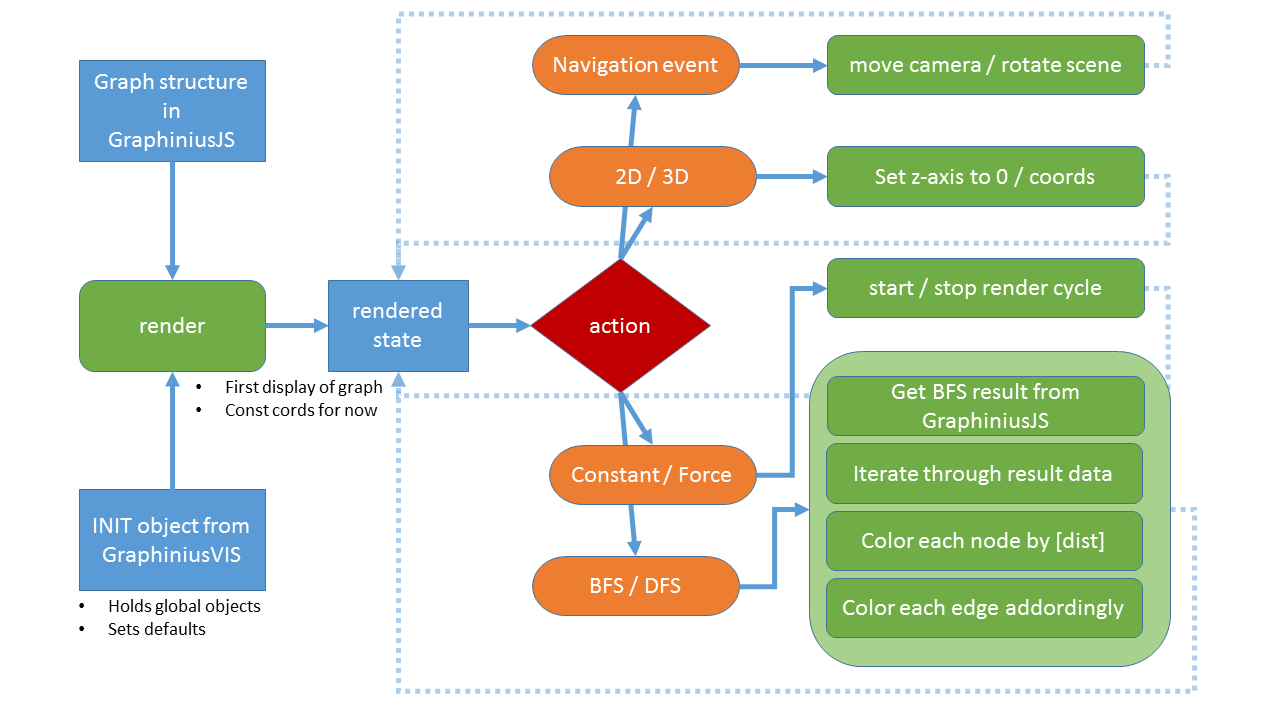
\includegraphics[width=1.2\textwidth]{figures/VIS_Control_Flow}
			\caption{Graphinius VIS control flow}
			\label{fig_vis_control_flow}
		\end{figure}
	%\end{landscape}


	
\section{Dependent Libraries}
\label{sect:dep_libraries}

	\begin{figure}[ht]
		\label{fig_dependencies}
		\centering
		\hspace*{-0.5cm}
		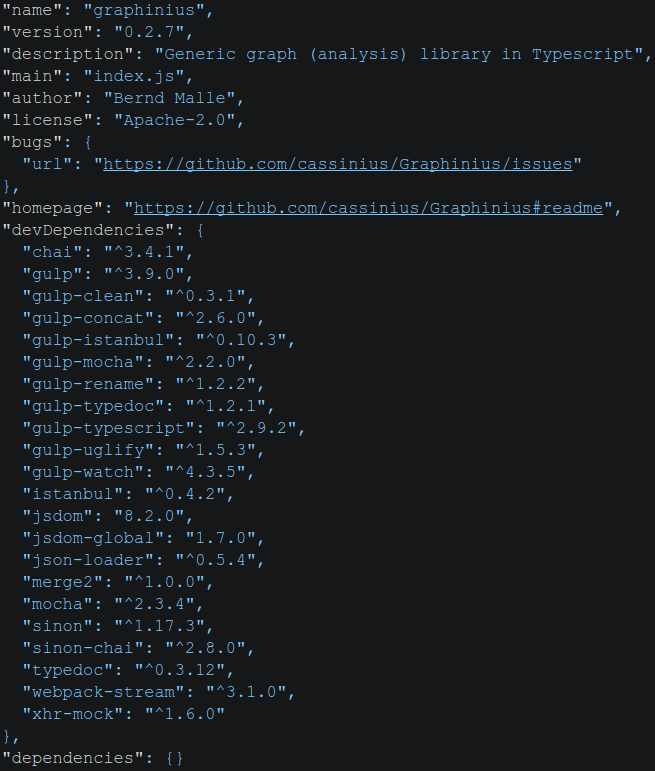
\includegraphics[width=0.8\textwidth]{figures/package_deps}
		\caption{GraphiniusJS development and runtime dependencies}
		\small
		As is clearly visible, I focused on managing all complexity during development time, resulting in zero dependencies for the runtime JS bundle.
	\end{figure}



\section{Testing approach}
\label{sect:testing_approach}

	BDD...
	
	\subsection{Unit tests}
	\label{ssect:unittests}
	
	\subsection{Functional tests}
	\label{ssect:func_tests}
	
	\subsection{Mocks used for browser code testing}
	\label{ssect:mocks}

	\subsection{Spies (Sinon)}
	\label{ssect:spies}


\section{Implemented Algorithms}
\label{sect:implemented_algos}

	\subsection{Degree Distribution}
	\label{ssect:deg_dist}

	\subsection{Core Search - Graph Traversal}
	\label{ssect:core_search}
	
		\subsubsection{Breadth first search}
		\label{sssect:search_bfs}
		
		\subsubsection{Depth first search}
		\label{sssect:search_dfs}
		
		\subsubsection{Best (priority) first search}
		\label{sssect:search_pfs}
		
		\subsubsection{Traversal-based algorithms}
		\label{sssect:travseral_algos}
		
		Centralities are 
	
	
\section{Platform Services}
\label{sect:platform_services}

As of the time of this writing, the Graphinius Platform has not taken shape yet, so there is no available implementation to discuss.

%\subsection{Personal Profile}
%\label{ssect:service_profile}

%\subsection{Teams}
%\label{ssect:service_teams}

%\subsection{Output / Reports}
%\label{ssect:service_output}